\section{Zadanie 6} 
Obserwator pełnego rzędu można obliczyć poleceniem:
\begin{minted}{matlab}
 Ld = acker(Ad',Cd',[zo1 zo2 zo3])'
\end{minted}
gdzie \mintinline{matlab}{zo1}, \mintinline{matlab}{zo2} i \mintinline{matlab}{zo3} to bieguny obserwatora. Wynik jest:
\begin{minted}{matlab}
 Ld =

    3.2279
   -1.4493
    0.1738
\end{minted}

Ponieważ obserwator jest programem komputerowym, można ustawić te bieguny na najszybsze z możliwych, czyli 0. Powstałe równania obserwatora to:
\[
\left\{
\begin{array}{l}
\hat{x}_1(k+1) = 3,23 \hat{x}_1(k) + \hat{x}_2(k) + 0,26 u(k) + 3,23(y(k) - \hat{x}_1(k)) \\
\hat{x}_2(k+1) = -1,45 \hat{x}_1(k) + \hat{x}_3(k) - 0,29 u(k) - 1,45(y(k) - \hat{x}_1(k)) \\
\hat{x}_3(k+1) = 0,17 \hat{x}_1(k) - 0,08 u(k) + 0,17(y(k) - \hat{x}_1(k)) \\
\end{array}
\right.
\]

\begin{figure}[H]
\centering
 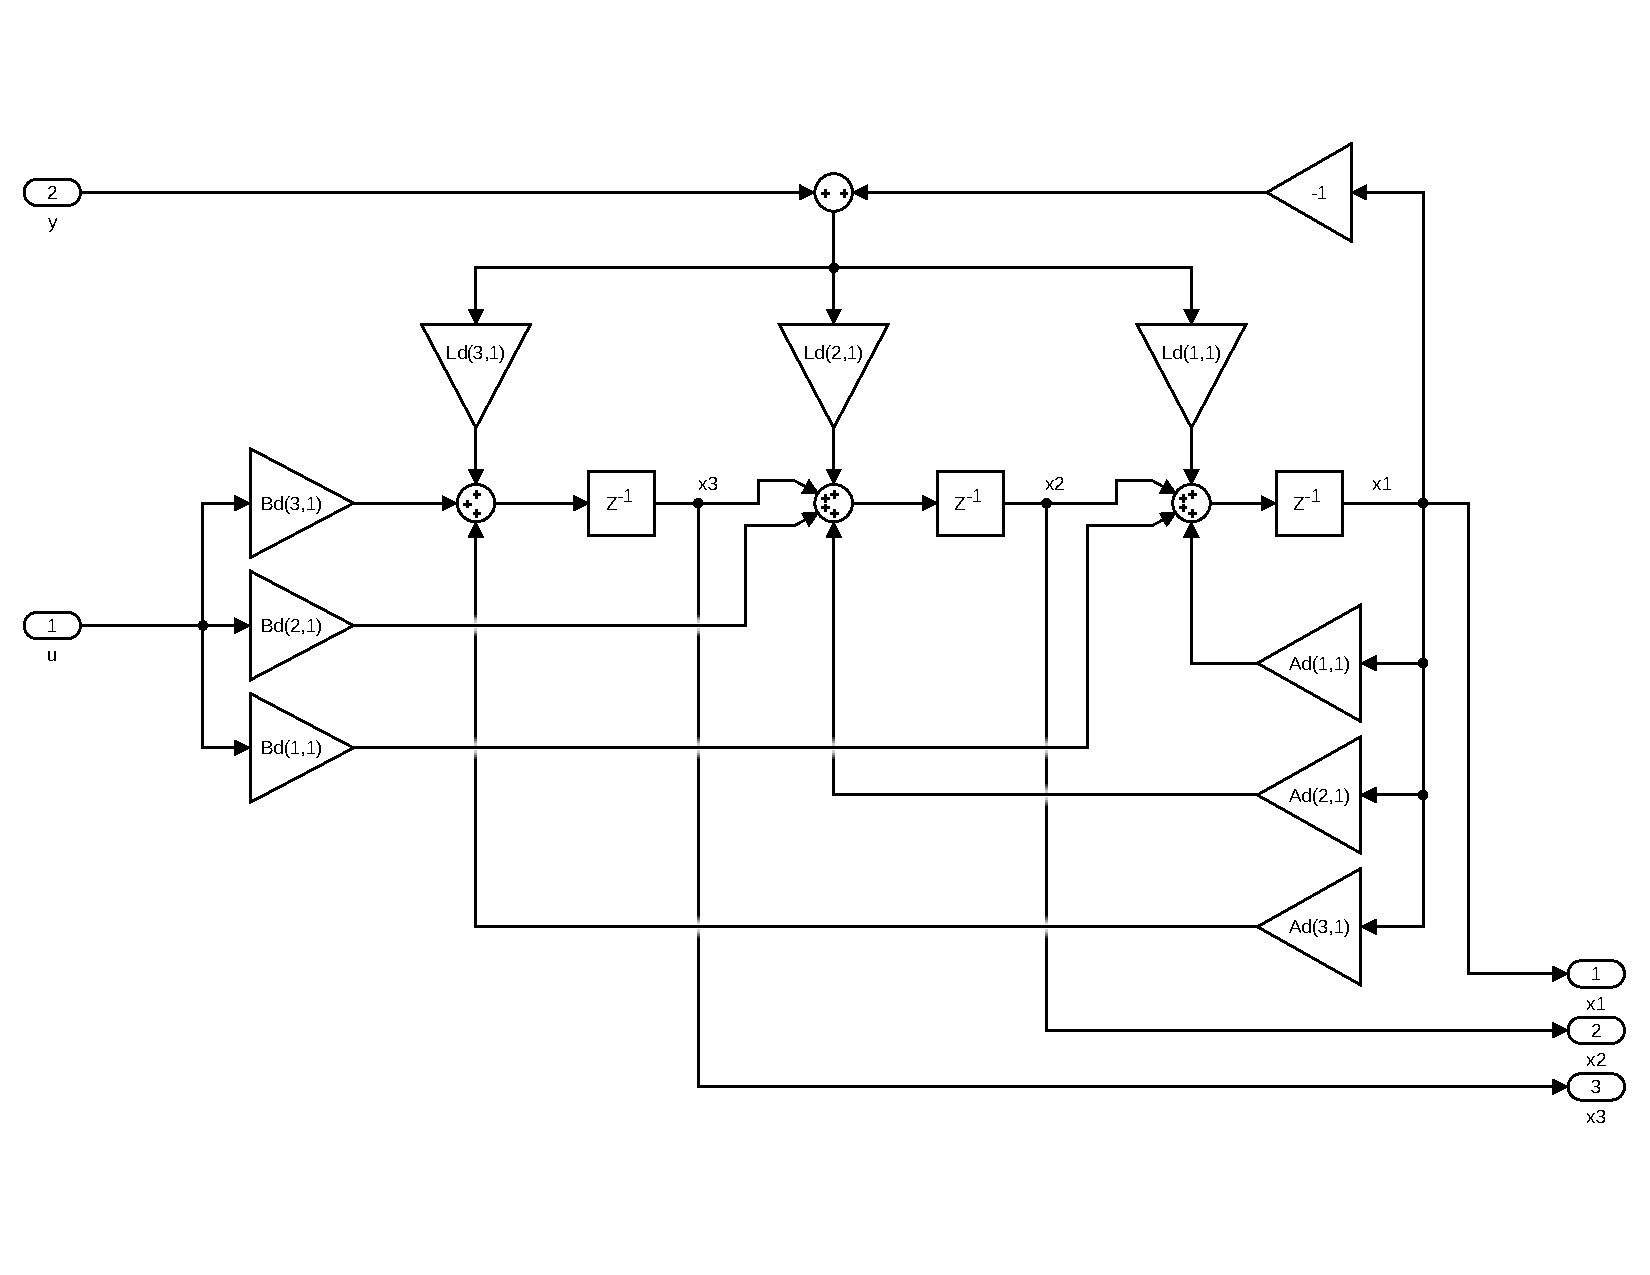
\includegraphics[width=\textwidth]{img/obs.pdf}
\caption{Obserwator pełnego rzędu.}
\end{figure}

\begin{figure}[H]
\centering
 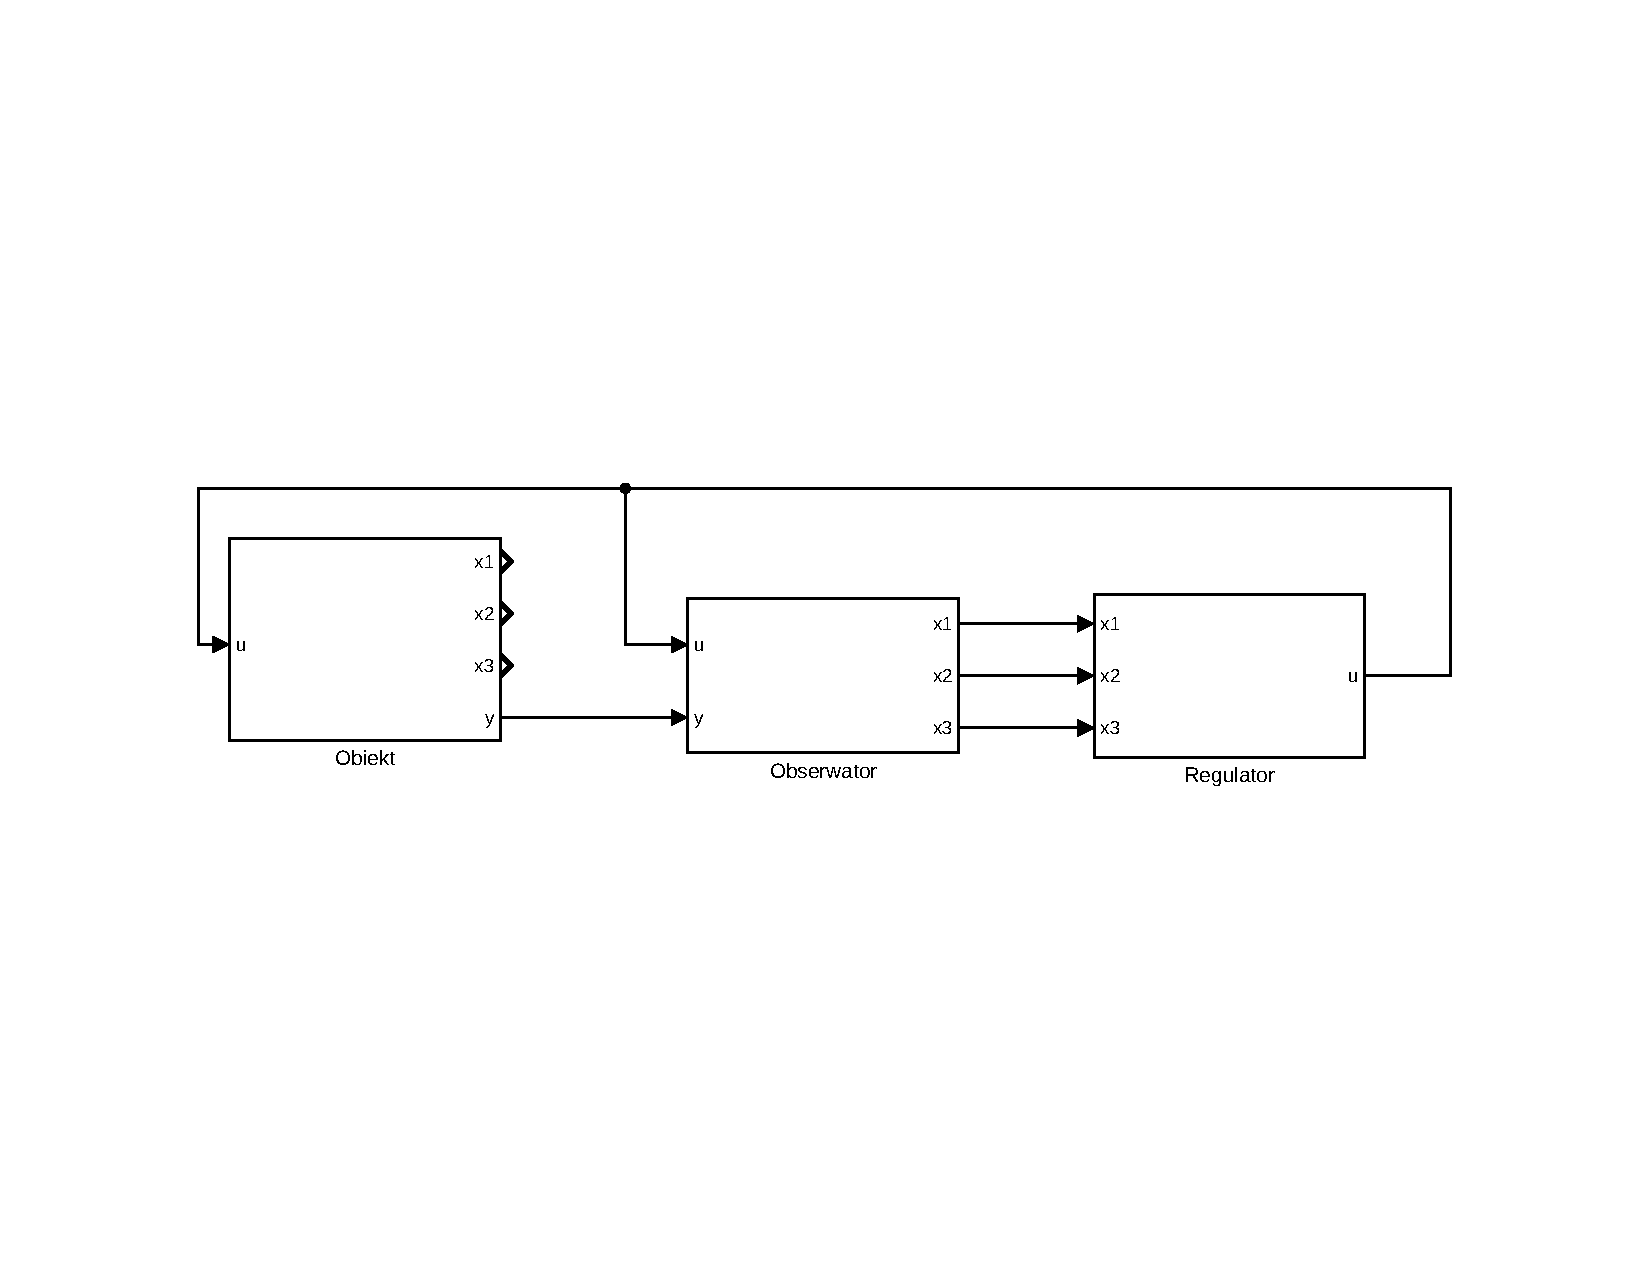
\includegraphics[width=\textwidth]{img/objobsreg.pdf}
\caption{Układ obiektu, obserwatora i regulatora.}
\end{figure}